\documentclass[numerate]{cheatsheet}
\usepackage{bm}
\usepackage{textcomp, mathcomp}
\usepackage{pbox}
\usepackage{amsmath, amssymb, mathtools, empheq, physics}
\usepackage{xcolor}
\usepackage{graphicx}
\usepackage{tikz}
\usepackage{pgfplots}
\usepackage{mathdots}
\usepackage{yhmath}
\usepackage{cancel}
\usepackage{color}
\usepackage{siunitx}
\usepackage{array}
\usepackage{multirow}
\usepackage{amssymb}
\usepackage{gensymb}
\usepackage{tabularx}
\usepackage{extarrows}
\usepackage{booktabs}

\usetikzlibrary{fadings}
\usetikzlibrary{patterns}
\usetikzlibrary{shadows.blur}
\usetikzlibrary{shapes}

\doctitle{Analysis 2 Zusammenfassung}
\author{Micha Bosshart - bmicha@ethz.ch \\ \vspace*{0.2em} \normalsize{ergänzt von Noa Sendlhofer \& Christian Leser} \vspace*{-0.2em}}

\begin{document}
    \section{Funktionen}
        \input{src/1_Funktionen/1_folgen-reihen.tex}
        \subsection{Grenzwerte}
    \subsubsection{Bernoulli de L'H$\hat{\textrm{o}}$pital}
        Falls $\displaystyle \lim_{x \to a} f(x) = \lim_{x \to a} g(x) = 0$ (oder $\pm \infty$), so gilt
        $$
            \lim_{x \to a} \frac{f(x)}{g(x)} = \lim_{x \to a} \frac{f'(x)}{g'(x)}.
        $$
    \subsubsection{Landau Symbol}
        \vspace{-0.5em}
        \begin{align*}
            \fbox{$f(x) = o(g(x)) \textrm{ für } x \to a$} &\Longleftrightarrow \lim_{x \to a} \frac{f(x)}{g(x)} = 0\\[0.5em]
            \fbox{$f(x) = O(g(x)) \textrm{ für } x \to a$}  &\Longleftrightarrow \lim_{x \to a} \left\lvert\frac{f(x)}{g(x)}\right\rvert \leq A \in \mathbb{R}
        \end{align*}
        $\textbf{Es gilt:}$
            \begin{align*}
                x^k &= o(e^x) \quad \textrm{ für } x \to \infty, \quad k \in \mathbb{R}\\
                \ln(x) &= o(x^k) \quad \textrm{ für } x \to \infty, \quad k > 0\\[0.5em]
                f(x) &= o(g(x)) \; \Rightarrow \; f(x) = O(g(x))\\
                f(x) &= O(g(x)) \; \nRightarrow \; f(x) = o(g(x))
            \end{align*}
    \subsection{Eigenschaften}
        Eine Funktion $f : A \to B$ ist eine Vorschrift, die jedem $x \in A$ ein Element $f(x) \in B$ zuordnet, $f: x \to f(x)$.
        \begin{description}
            \item[Definitionsbereich:] $D(f) = A$
            \item[Zielbereich:] $Z(f) = B$
            \item[Wertebereich:] $W(f) = \{ f(x) \vert \ x \in D(f)\}$   
        \end{description}
        \subsubsection{Surjektiv}
            Jeder Wert im Zielbereich $Z(f)$ wird angenommen.
            \mathbox{
                W(f) = Z(f)
            }
        \subsubsection{Injektiv}
            Jede Horizontale schneidet den Graphen $\Gamma(f)$ höchstens einmal.
            \begin{itemize}
                \item $f(x_1) = f(x_2) \Rightarrow x_1 = x_2$, sonst nicht injektiv
            \end{itemize}
        \subsubsection{Bijektiv}
            \begin{center}
                Injektiv \& Surjektiv $\Leftrightarrow$ Bijektiv $\Leftrightarrow$ Umkehrbar
            \end{center}
        \subsubsection{Inverse Funktion}
            Sei $f(x)$ eine Funktion von $D(f)$ nach $W(f)$, dann ist $f^{-1}: W(f) \to D(f)$ mit $y \mapsto f^{-1}(y)$ die inverse Funktion von $f(x)$.
            \begin{itemize}
                \item $W(f^{-1}) = D(f)$
                \item $D(f^{-1}) = W(f)$
            \end{itemize}
        \subsubsection{Gerade \& Ungerade}
            \begin{description}
                \item[gerade:]\phantom{as} $f(-x) = f(x)$ 
                \item[ungerade:] $f(-x) = -f(x)$ 
            \end{description}
        \subsubsection{Stetigkeit}
            $f(x)$ ist stetig im Punkt $\xi$ falls
            $$
                \lim_{x\to\xi^-} f(x) = f(\xi) = \lim_{x\to\xi^+} f(x).
            $$
            \begin{itemize}
                \item Bei Lücken in $D(f)$ werden die einzelnen Abschnitte separat betrachtet.
            \end{itemize}
        \subsubsection{Monotonie}
            \textbf{(Strikt) Monoton Steigend}
                \begin{itemize}
                    \item $x_1 < x_2\ \Longleftrightarrow\ f(x_1) \leq f(x_2)$ \hfill (strikt: $<$)
                    \item $f'(x) \geq 0$ \hfill (strikt: $>$)
                \end{itemize}
            \textbf{(Strikt) Monoton Fallend}
                \begin{itemize}
                    \item $x_1 < x_2\ \Longleftrightarrow\ f(x_1) \geq f(x_2)$ \hfill (strikt: $>$)
                    \item $f'(x) \leq 0$ \hfill (strikt: $<$)
                \end{itemize}
        \subsubsection{Beschränktheit}
            Alle Funktionswerte sind in einem endlich breiten waagerechten Parallelstreifen enthalten.
        \input{src/1_Funktionen/3_asymptoten.tex}
        % !TeX root = ../../ZF_bmicha_Ana.tex
\subsection{Hyperbolische Funktionen}
    $$ \cosh(x) = \frac{e^x + e^{-x}}{2} \qquad \sinh(x) = \frac{e^x - e^{-x}}{2}$$
    $$
        \tanh(x) = \frac{\sinh(x)}{\cosh(x)}
    $$
    $$
        \frac{d}{dx} \cosh(x) = \sinh(x) \qquad \frac{d}{dx} \sinh(x) = \cosh(x)
    $$
    $$
        \cosh(x)^2 - \sinh(x)^2 = 1
    $$

    \subsubsection{Inverse Funktionen}
        \begin{align*}
            \cosh(x)^{-1} &= \textrm{arcosh}(x) &= \ln(x + \sqrt{x^2 - 1})\\
            \sinh(x)^{-1} &= \textrm{arsinh}(x) &= \ln(x + \sqrt{x^2 + 1})\\
            \tanh(x)^{-1} &= \textrm{artanh}(x) &= \frac{1}{2} \ln(\frac{1+x}{1-x})
        \end{align*}

    \section{Komplexe Zahlen}
        \input{src/2_Komplexe_Zahlen/1_basics.tex}
        \input{src/2_Komplexe_Zahlen/2_nullstellen-reeller-Polynome.tex}
        \subsection{Komplex Konjugierte}
    \begin{align*}
        \text{Komplexe Zahl: } z = x - iy\\
        \text{Komplex konjugierte Zahl: } \bar{z} = x -iy\\
    \end{align*}
    \vspace{-2em}
    \[\begin{array}{c | c}
        \frac{z_1}{z_2} = \frac{z_1 \cdot \bar{z_2}}{z_2 \cdot \bar{z_2}} & \frac{1}{z^2 - 1} = \frac{\bar{z}^2 -1}{|z^2 - 1|}
    \end{array}\]
    \section{Potenzreihen}
        % !TeX root = ../../ZF_bmicha_Ana.tex
\vspace{0.5em}
Potenzreihe der Funktion $f(x)$ um den Punkt $x_o$:
\mathbox{
    f(x) = \sum_{n=0}^{\infty} a_n \cdot (x-x_o)^n
}
\vspace{-1.0em}
\begin{itemize}
    \item Höchstens eine Potenzreihe von $f$ um $x_o$ existiert.
    \item Konvergiert für $\abs*{x-x_o} < r$
\end{itemize}
\vspace{-1em}
\mathbox{
    \frac{1}{1 - \fcolorbox{green}{white}{x}} = \sum\limits_{n = 0}^{\infty} \fcolorbox{green}{white}{x}^k
}
\vspace{-0.5em}
        \input{src/3_Potenzreihen/2_konvergenzradius.tex}
        \input{src/3_Potenzreihen/3_taylorreihen.tex}
    \section{Trigonometrie}
        \input{src/4_Trigonometrie/1_tabelle.tex}
        % \subsection{Einheitskreis}
    \centerline{
        \resizebox{4cm}{4cm}{
            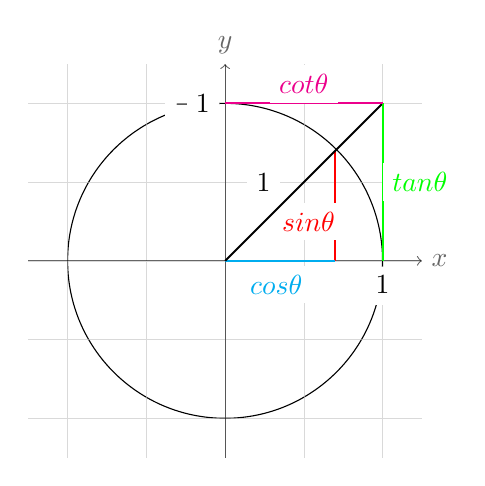
\begin{tikzpicture}
                %circle
                \draw[smooth, samples = 600] (0, 0) circle (2)(1, 1);
                
                % coordinate system
                \draw[opacity=0.6,lightgray,very thin,step=1cm](-2.5,-2.5) grid (2.5,2.5);
                \draw[->,opacity=0.6](-2.5,0) -- (2.5,0) node [right]{$x$};
                \foreach \x in {-1,...,1}
                \draw[xshift=2cm] (0,2pt) -- (0,-2pt) node[below,fill=white]{$\x$};
                \draw[->,opacity=0.6](0,-2.5) -- (0,2.5) node[above]{$y$};
                \foreach \y in {-1,...,1}
                \draw[yshift=2cm] (2pt,0) -- (-2pt,0) node[left,fill=white] {$\y$};
                
                %sin
                \draw[line width=0.25mm,red] (1.39, 1.39) -- (1.39,0);
                    \draw (0.6,0.5) node[red,right,fill=white] {$sin\theta$};
                %cos
                \draw[line width=0.25mm,cyan] (0, 0) -- (1.39, 0);
                    \draw (0.65,-0.3) node[cyan,fill=white] {$cos\theta$};
                %Hypotenuse
                \draw[line width=0.25mm,black] (0, 0) -- (2, 2);
                    \draw (0.7,1) node[left, black,fill=white] {$1$};
                %tan
                \draw[line width=0.25mm,green] (2,0) -- (2, 2);
                    \draw (2, 1) node[green, right, fill=white] {$tan\theta$};
                %cot
                \draw[line width=0.25mm,magenta] (2, 2) -- (0, 2);
                    \draw (1, 2) node[magenta, above, fill=white] {$cot\theta$};
                
            \end{tikzpicture}
        }
    }
    \vspace*{0.5em}
        \input{src/4_Trigonometrie/3_rechenregeln.tex}
        \input{src/4_Trigonometrie/4_funktionsmodifikation.tex}
    \section{Parametrisierungen}
        % !TeX root = ../../ZF_bmicha_Ana.tex
\subsection{Kreis / Ellipse}
    Ellipse mit Mittelpunkt $(x_o, y_o)$ und Halbachsen $a$ \& $b$.\\
    \underline{\textit{implizit}:}
    $$
        \left(
            \frac{x-x_o}{a}
        \right)^2
        +
        \left(
            \frac{y-y_o}{b}
        \right)^2
        = 1
    $$
    \underline{\textit{parametrisiert}:}
    \begin{align*}
        x(t) &= x_o + a \cdot \cos(t)\\
        y(t) &= y_o + b \cdot \sin(t)
    \end{align*}

\subsection{Hyperboloid}
    \underline{\textit{implizit}:}
    $$
    \left(
        \frac{x-x_o}{a}
    \right)^2
    +
    \left(
        \frac{y-y_o}{b}
    \right)^2
    +
    \left(
        \frac{z-z_o}{c}
    \right)^2
    = 1
    $$

    \underline{\textit{parametrisiert}:}
    \begin{align*}
        x(\lambda, t) &= a(\cos(t) - \lambda \sin(t))\\
        y(\lambda, t) &= b(\sin(t) + \lambda \cos(t))\\
        z(\lambda, t) &= c\lambda
    \end{align*}
        \subsection{Normal- und Tangentialvektoren}
    \subsubsection{explizit}
    $$
            y = f(x)
        \quad
            \vec{t} = \begin{pmatrix}
                1\\f'(x_o)
            \end{pmatrix}
        \quad 
            \vec{n} = \begin{pmatrix}
                f'(x_o) \\ -1
            \end{pmatrix}
    $$
    \vspace*{-0.25em}
    \subsubsection{parametrisiert}
    $$
            \vec{r}(t) = \begin{pmatrix}
                x(t)\\y(t)
            \end{pmatrix}
        \quad 
            \vec{t} = \begin{pmatrix}
                \dot{x}(t)\\ \dot{y}(t)
            \end{pmatrix}
        \quad 
            \vec{n} = \begin{pmatrix}
                -\dot{y}(t)\\ \dot{x}(t)
            \end{pmatrix}
    $$
    \section{Differentialrechnung}
        % !TeX root = ../../ZF_bmicha_Ana.tex
\subsection{Ableitung Inverse Funktion}
    $$
        (f^{-1})'(x_o) = \frac{1}{f'(f^{-1}(x_o))}
    $$
        % !TeX root = ../../ZF_bmicha_Ana.tex
\subsection{Tangenten}
    \subsubsection{Explizit}
        \vspace*{0.5em}
        \mathbox{
            t(x) = f(x_o) + f'(x_o) \cdot (x-x_o)
        }
        Eine Tangente $t(x)$ an die Funktion $f(x)$ im Punkt $x_o$, erfüllt folgende Bedingungen:
        \begin{align*}
            t'(x_o) & \overset{!}{=} f'(x_o),\\
            t(x_o) & \overset{!}{=} f(x_o).
        \end{align*}
    \subsubsection{Parametrisiert}
        Tangente $\vec{t}(s)$  an die Parametrisierung $\vec{r}(t)$ im Punkt $t_o$.
        \mathbox{
            \vec{t}(s) = \begin{pmatrix}
                x(s)\\ y(s)
            \end{pmatrix}
            = \vec{r}\ (t_o) + s \cdot \dot{\vec{r}}\ (t_o)
        }
        % !TeX root = ../../ZF_bmicha_Ana.tex
\subsection{Fehlerrechnung}
    Die berechnete Grösse $f$ ist abhängig von der gemessenen Grösse $x$.
    Die gemessene Grösse weicht mit dem Messfehler $dx$ von der Realität ab.
    \begin{itemize}
        \item \textbf{Linearisierung}
            \vspace*{-0.5em}
            \mathbox{
                f(x) \approx  f(x_0) + \left. \frac{\partial f}{\partial x} \right|_{x_0} \cdot (x - x_0)
            }
        \item \textbf{Absoluter Fehler}
            \vspace*{-0.5em}
            \mathbox{
                \Delta f = f(x + \Delta x) -\! f(x) \quad \overset{\Delta x \to 0}{\longrightarrow} \quad \Delta f \approx f'(x)\ \Delta x
            }
        \item \textbf{Relativer Fehler}
            \vspace*{-0.5em}
            \mathbox{
                \frac{df}{f}
            }
    \end{itemize}
    \subsubsection{Bemerkungen}
        \vspace{0.5em}
        \begin{minipage}{0.54\linewidth}
            \centering \vspace{4pt}
            $1\%$ Genauigkeit
            $$
                \frac{\Delta x}{x} = 1\% = \frac{1}{100}
            $$          
        \end{minipage}
        \begin{minipage}{0.45\linewidth}
            \centering
            Messfehler von $1^\circ$
            $$
                \Delta \alpha = \frac{\pi}{180}
            $$
        \end{minipage}
        \input{src/10_Differentialrechnung/4_evolute.tex}
        % !TeX root = ../../ZF_bmicha_Ana.tex
\subsection{Krümmung \hfill $k(t)$}
    \begin{itemize}
        \item Parametrisierung $\vec{r}(t) = (x(t),y(t))^T$
            $$
                k(t) = \frac{\dot{x} \ddot{y} - \ddot{x} \dot{y}}{\left( \dot{x}^2 + \dot{y}^2 \right)^{\frac{3}{2}}}
            $$
        \item Explizit $y=f(x)$
            $$
                k(x) = \frac{f''(x)}{(1+f'(x)^2)^{3/2}}
            $$
        \item Polarkoordinaten $r=f(\varphi)$
            $$
                k(\varphi) = \frac{(f(\varphi))^2 + 2(f'(\varphi))^2-f(\varphi)f''(\varphi)}{\left[(f(\varphi))^2 + (f'(\varphi))^2\right]^{3/2}}
            $$
    \end{itemize}
    \section{Integralrechnung}
        \input{src/11_Integralrechnung/1_leibnitz.tex}
        % !TeX root = ../../ZF_bmicha_Ana.tex
\subsection{Hauptsatz der Infinitesimalrechnung}
    Für $a \in \mathbb{R}$
    \mathbox{
        \frac{d}{dx} 
        \left[
            \int_a^x f(t) dt
        \right]
        = f(x)
    }
        \input{src/11_Integralrechnung/3_partialbruchzerlegung.tex}
        % !TeX root = ../../ZF_bmicha_Ana.tex
\subsection{Partielle Integration}
    Es sei $F'(x) = f(x)$ und $G'(x) = g(x)$, dann gilt
    $$
        \int_a^b \underset{\downarrow}{G} \cdot \underset{\uparrow}{f} \, dx = G \cdot F \Big\rvert_a^b - \int_a^b g \cdot F \, dx.
    $$
        % !TeX root = ../../ZF_bmicha_Ana.tex
\subsection{Bogenlänge \hfill $s\ $}
    \begin{itemize}
        \item explizit $y = f(x)$
            $$
                s = \int_a^b \sqrt{1 + \left( f'(x) \right)^2} \ dx
            $$
        \item Polarkoordinaten $\rho = \rho(\varphi)$
            $$
                s = \int_{\varphi_1}^{\varphi_2} \sqrt{\rho^2 + \dot{\rho}^2} \ d\varphi
            $$
        \item Parametrisierung $\vec{r}(t) = (x(t),y(t))^T$
            $$
                s = \int_{t_1}^{t_2} \left\lvert \sqrt{\dot{x}^2 + \dot{y}^2} \right\rvert \ dt
            $$
    \end{itemize}
        \input{src/11_Integralrechnung/6_flaechenberechnungen.tex}
        % !TeX root = ../../ZF_bmicha_Ana.tex
\subsection*{Rotationsvolumen}
    \subsubsection*{Kurvenrotation}
        \underline{Kurve rotiert um x-Achse:}
        $$
        V = \int_{t_1}^{t_2} \pi y^2(t) \cdot \underbrace{\dot{x}(t) dt}_{dx} = \int_{x_1}^{x_2} \pi f^2(x) \cdot dx
        $$
        \underline{Kurve rotiert um y-Achse:}
        $$
        V = \int_{t_1}^{t_2} \pi x^2(t) \cdot \underbrace{\dot{y}(t) dt}_{dy} = \int_{y_1}^{y_2} \pi x^2 \cdot \underbrace{f'(x) dx}_{dy}
        $$

    \subsubsection*{Flächenrotation}
        \underline{Fläche unter Kurve rotiert um $y$-Achse:}
        $$
        V = \int_{t_1}^{t_2} \underbrace{2\pi x(t)}_{\textrm{Umfang}} \cdot y(t) \cdot \underbrace{\dot{x}(t) dt}_{dx} = \int_{x_1}^{x_2} 2\pi x \cdot f(x) dx
        $$


        % !TeX root = ../../ZF_bmicha_Ana.tex
\subsection{Rotationsoberflächen}
    \underline{Kurve rotiert um x-Achse:}
    \begin{align*}
        O &= \int_{t_1}^{t_2} 2 \pi y(t) \cdot \underbrace{\sqrt{\dot{x}^2(t) + \dot{y}^2(t)}\ dt}_{ds \textrm{ (Bogenlänge)}}\\
          &= \int_{x_1}^{x_2} 2 \pi f(x) \cdot \underbrace{\sqrt{1 + f'(x)^2}\ dt}_{ds}
    \end{align*}
    \underline{Kurve rotiert um y-Achse:}
    \begin{align*}
        O &= \int_{t_1}^{t_2} 2 \pi x(t) \cdot \underbrace{\sqrt{\dot{x}^2(t) + \dot{y}^2(t)}\ dt}_{ds}\\
          &= \int_{x_1}^{x_2} 2 \pi x \cdot \underbrace{\sqrt{1 + f'(x)^2}\ dx}_{ds}
    \end{align*}

        % % !TeX root = ../../ZF_bmicha_Ana.tex
\subsection{Schwerpunkt / Trägheitsmoment}
    Sei $H(x)$ die Höhe des Fläche a.d.S. $x$.\\
    Sei $\sigma$ die Flächendichte $[kg/m^2]$.
    \begin{align*}
        \textrm{Fläche: }  A = \int_{x_1}^{x_2} H(x)\ dx\\
        \textrm{Masse: }  M = \int_{x_1}^{x_2} \sigma \cdot H(x)\ dx\\
        \textrm{Schwerpunkt: }  x_s = \frac{1}{M} \int_{x_1}^{x_2} x \cdot \sigma \cdot H(x)\ dx\\
        \textrm{SP Rotationsvolumen: } x_s = \frac{1}{V} \int_{x_1}^{x_2} x \cdot \pi \cdot H^2(x)\ dx\\
        \textrm{Trägheitsmoment: }  I_y = \int_{x_1}^{x_2} x^2 \cdot \sigma \cdot H(x)\ dx
    \end{align*}
    \subsubsection{Trägheitsmoment}
    \vspace*{-1em}
        \begin{align*}
            \Theta =& \int (\textrm{Abstand zur Rotationsachse})^2 \cdot (\textrm{Masse})\\
            \Theta =& \; \rho \cdot \int_a^b x^2 \cdot G(x) dx\\
            J_0 =& \; \frac{\pi R^4}{2} = \; \parbox{5cm}{polares Flächenträgheitsmoment\\ der Kreisscheibe}\\
            \Theta_x =& \; \rho \cdot \int_a^b \frac{1}{2} \pi (f(x))^4 dx = \; \parbox{5cm}{Masseträgheitsmoment\\ eines Rotationskörpers\\ um die x-Achse}\\
            \Theta =& \; \rho \cdot \frac{1}{2} \pi \int_a^{b} y(t)^4\|\dot{x}(t)\| dt\\
            G(x) =& \; \text{Masse an diesem Abstand}\\
            M(x) =& \; \text{Mantelfäche} = 2 \pi x \cdot G(x) = \text{Umfang} \cdot \text{Höhe}\\ %\underbrace{2 \pi x \vphantom{G(x)}}_{\text{Umfang}} \cdot \underbrace{G(x)}_{\text{Höhe}}\\
            \Theta_z =& \; \rho \int_{x_1}^{x_2} x^2 \cdot M(x) dx
        \end{align*}        
        \input{src/11_Integralrechnung/10_uneigentliche-integrale.tex}
        \vfill \null \columnbreak

    \section{Mehrdimensionale Fkt. - Diff. Rechnung}
        % !TeX root = ../../ZF_bmicha_Ana.tex
\subsection{Fehlerrechnung}
    Die berechnete Grösse $f$ ist abhängig von den gemessenen Grössen $x,y$.
    Die gemessenen Grössen weichen mit den Messfehlern $dx,dy$ von der Realität ab.
    \begin{itemize}
        \item \textbf{Totales Differential / Absoluter Fehler}
            \mathbox{
                df \approx f_x\ dx + f_y\ dy
            }
        \item \textbf{Relativer Fehler}
            \mathbox{
                \frac{df}{f}
            }
    \end{itemize}
    \subsubsection{Bemerkungen}
        \vspace{0.5em}
        \begin{minipage}{0.54\linewidth}
            \centering \vspace{4pt}
            $1\%$ Genauigkeit
            $$
                \frac{dx}{x} = 1\% = \frac{1}{100}
            $$          
        \end{minipage}
        \begin{minipage}{0.45\linewidth}
            \centering
            Messfehler von $1^\circ$
            $$
                d\alpha = \frac{\pi}{180}
            $$
        \end{minipage}
        \input{src/5_Mehrdimensionale-Funktionen_Differentialrechnung/2_niveaulinien-flaechen.tex}
        \input{src/5_Mehrdimensionale-Funktionen_Differentialrechnung/3_gradient.tex}
        \input{src/5_Mehrdimensionale-Funktionen_Differentialrechnung/4_richtungsableitung.tex}
        % !TeX root = ../../ZF_bmicha_Ana.tex
\subsection{Tangentialebenen}
    \subsubsection{Linearisierungsformel}
        \mathbox{
            z = f(x_o,y_o) + f_x(x_o,y_o) (x\!-\!x_o) + f_y(x_o,y_o)(y\!-\!y_o)
        }
        \mathbox{
            0 = f_x(x_o,y_o,z_o)(x\!-\!x_o) + f_y(x_o,y_o,z_o)(y\!-\!y_o) + \dots
        }
    \subsubsection{Gradient}
        \begin{itemize}
            \item $f(x,y,z) = C$ ist eine Niveaufläche
            \item $\grad(f)$ steht senkrecht auf Niveauflächen. ($\to \vec{n}$ )
            \item Ebene mit Normalenvektor $\vec{n}= (A,B,C)^T$:
            $$
                Ax + By + Cz = D
            $$
        \end{itemize}
        % !TeX root = ../../ZF_bmicha_Ana.tex
\subsection{Extremalstellen von $f(x,y)$}
    \vspace{0.25em}
    \begin{enumerate}
        \item Inneres untersuchen $\to$ $\textrm{grad}f \overset{!}{=} 0$
        \item Rand untersuchen
        \begin{itemize}
            \item Lagrange Multiplikatoren
            \begin{enumerate}
                \item $g(x,y)$ beschreibt Rand
                \item $\textrm{grad}f(x_o,y_o) = \lambda \cdot \textrm{grad}\, g(x_o,y_o)$\\[0.25em]
                      \phantom{llll}$\textrm{grad}\, g(x_o,y_o) \neq 0,\phantom{ll} \lambda \in \mathbb{R}$
                \item Gleichungssystem aus (a) und (b) lösen.
            \end{enumerate}
            \item Parametrisierung
            \begin{enumerate}
                \item Rand parametrisieren
                \item Parametrisierung in $f$ einsetzen
                \item Nach Parameter ableiten und nullsetzen.\\[0.25em] \phantom{llll}$f'(t) = 0$
            \end{enumerate}
        \end{itemize}
        \item Eckpunkte untersuchen
        \item Kandidaten vergleichen
        \item Art der Extremalstelle: Hesse-Matrix aufstellen $\mathcal{H} = 
        \left[
            \begin{array}{c c} 
                \frac{\partial^2 f}{\partial x^2}       & \frac{\partial^2 f}{\partial x \partial y}\\
                \frac{\partial^2 f}{\partial x \partial y}  & \frac{\partial^2 f}{\partial y^2}
            \end{array}
        \right]$
            \begin{itemize}
                \item Maximum: $\mathcal{H}$ ist negativ definit ($\lambda_i < 0$)
                \item Minimum: $\mathcal{H}$ ist positiv definit ($\lambda_i > 0$)
                \item Sattelstelle: $\mathcal{H}$ ist indefinit ($\mathcal{H}$ besitzt $\lambda_i > 0$ \textbf{und} $\lambda_i < 0$)
            \end{itemize}
    \end{enumerate}
        \input{src/5_Mehrdimensionale-Funktionen_Differentialrechnung/7_satz-von-schwarz.tex}
        \input{src/5_Mehrdimensionale-Funktionen_Differentialrechnung/8_integrabilitaetsbedingung.tex}
        \input{src/5_Mehrdimensionale-Funktionen_Differentialrechnung/9_verallg_kettenregel.tex}
        \vfill \null \columnbreak
        
    \section{Mehrdimensionale Fkt. - Int. Rechnung}
        \input{src/6_Mehrdimensionale-Funktionen_Integralrechnung/1_doppel-und-dreifachintegrale.tex}
        \input{src/6_Mehrdimensionale-Funktionen_Integralrechnung/2_dimensionsvergleich.tex}
        \input{src/6_Mehrdimensionale-Funktionen_Integralrechnung/3_koordinatentransformationen.tex}
        % !TeX root = ../../ZF_bmicha_Ana.tex
\subsubsection{Ellipsenkoordinaten}
    \begin{minipage}{0.49\linewidth}
        \vspace{0.5em}
        \underline{\textbf{Rand:}}\\
        \textit{implizit:}
        $$
            \left( \frac{x}{a} \right)^2 + \left( \frac{y}{b} \right)^2 = 1
        $$
        \textit{parametrisiert:}
        \begin{align*}
            x &= a \cdot \cos(\varphi)\\
            y &= b \cdot \sin(\varphi)\\
        \end{align*}
    \end{minipage}
    \begin{minipage}{0.5\linewidth}
        \includegraphics[width=\linewidth]{src/6_Mehrdimensionale-Funktionen_Integralrechnung/ellipse.pdf}
    \end{minipage}\vspace{-1em}
    \begin{minipage}{0.49\linewidth}
        \textbf{\underline{Fläche:}}
            \begin{align*}
                x &= a \cdot r \cdot \cos(\varphi)\\
                y &= b \cdot r \cdot \sin(\varphi)
            \end{align*}
    \end{minipage}
    \begin{minipage}{0.5\linewidth}
        \vspace{0.8em}
        \begin{align*}
            dA &= abr \, dr d\varphi\\
            r &\in [0,1]
        \end{align*}
    \end{minipage}
        
        \input{src/6_Mehrdimensionale-Funktionen_Integralrechnung/5_jacobi.tex}
        % !TeX root = ../../ZF_bmicha_Ana.tex
\subsection{Schwerpunkte}
    \subsubsection{2D}
    $\sigma(x,y)$: Flächendichte $[kg/m^2 ] $
        \begin{align*}
            &m = \iint \sigma(x,y) \, dA\\[0.25em]
            x_s =&\, \frac{1}{m} \iint x \cdot \sigma(x,y) \, dA\\
            y_s =&\, \frac{1}{m} \iint y \cdot \sigma(x,y) \, dA
        \end{align*}
    \textit{Keine Angabe für $\sigma$: $\sigma = 1$}
    \subsubsection{3D}
    $\rho(x,y,z)$: Volumendichte $[kg/m^3 ] $
        \begin{align*}
            &m = \iiint \rho(x,y,z) \, dV\\[0.25em]
            x_s =&\, \frac{1}{m} \iiint x \cdot \rho(x,y,z) \, dV\\
            % y_s =&\, \frac{1}{m} \iiint y \cdot \rho(x,y,z) \, dV
            y_s =&\, \dots
        \end{align*}
        \vspace{-0.45em}
    \textit{Keine Angabe für $\rho$: $\rho = 1$}
    \vspace{0.5em}

        
        % !TeX root = ../../ZF_bmicha_Ana.tex
\subsection{Trägheitsmoment}
    \subsubsection{2D}
        \textbf{Trägheitsmoment bzgl. einer Achse:}
        \begin{align*}
            I_x =& \iint_A \sigma(x,y) \cdot y^2 \, dA\\
            I_y =& \iint_A \sigma(x,y) \cdot x^2 \, dA
        \end{align*}
        \textbf{Polares Trägheitsmom.} (bzgl. $z$-Achse/ Ursprung):
        \begin{align*}
            I_o = I_x + I_y = \iint_A \sigma(x,y) \cdot (x^2 + y^2) \, dA 
        \end{align*}
        \textit{Keine Angabe für $\sigma$: $\sigma = 1$}

    \subsubsection{3D}
        \textbf{Trägheitsmoment bzgl. Achse:}
        \begin{align*}
            I_x =& \iiint_V \rho(x,y,z) \cdot (y^2 + z^2) \, dV\\
            I_y =& \iiint_V \rho(x,y,z) \cdot (x^2 + z^2) \, dV
        \end{align*}
        \textit{Keine Angabe für $\rho$: $\rho = 1$}
        
    \subsubsection{Satz von Steiner}
    \begin{minipage}{0.5\linewidth}
        \includegraphics[width=\linewidth]{src/6_Mehrdimensionale-Funktionen_Integralrechnung/satz-von-steiner.pdf}
    \end{minipage}
    \hspace{0.05\linewidth}
    \begin{minipage}{0.4\linewidth}
        \begin{align*}
            I_p &=\,\, I_s + d^2 \cdot m\\
            m \vcentcolon&= Masse\\
            d \vcentcolon&= Abstand\\
        \end{align*}
    \end{minipage}
        % !TeX root = ../../ZF_bmicha_Ana.tex
\subsection{Leibnitz Theorem}
$$
    \frac{d}{dx} \left( \int_{a(x)}^{b(x)} f(x,t) dt \right) =
$$
$$
    \int_{a(x)}^{b(x)}  f_x(x,t) dt + f(x,b(x)) \, \frac{db(x)}{dx}  - f(x,a(x)) \, \frac{da(x)}{dx}
$$
\vspace{0.9em}

        % !TeX root = ../../ZF_bmicha_Ana.tex
\subsection{Oberflächenintegrale}
    Spezialfall eines Flächenintegrals.\\    
    Flächeninhalt einer parametr. Oberfläche berechnen:
    \mathbox{
        \iint_{\mathcal{O}} d\mathcal{O} = \iint_{\mathcal{O}} \abs*{\vec{r}_u \times \vec{r}_v} du dv
    }
    \textbf{Parametrisierung der Oberfläche:}
    $$
        \vec{r} = \begin{pmatrix}
            x(u,v)\\
            y(u,v)\\
            z(u,v)
        \end{pmatrix}
    $$
    \vspace*{0.0em}
    \begin{description}
        \item[Oberflächenelement:] $d\mathcal{O} = \abs*{\vec{r}_u \times \vec{r}_v} du dv$
        \item[Normalenvektor:]  $\vec{n} = \vec{r}_u \times \vec{r}_v$
        \item[Normaleneinheitsvektor:]  $\vec{n}_o = \frac{\vec{r}_u \times \vec{r}_v}{\abs*{\vec{r}_u \times \vec{r}_v}}$
    \end{description}
    {\small Oberflächenelement entspricht Jacobi-Determinante.}
        \input{src/6_Mehrdimensionale-Funktionen_Integralrechnung/10_parametrisierungen-flaechen.tex}
        \vfill \null \columnbreak

    \section{Vektoranalysis}
        % !TeX root = ../../ZF_bmicha_Ana.tex
\vspace{0.5em}
Potenzreihe der Funktion $f(x)$ um den Punkt $x_o$:
\mathbox{
    f(x) = \sum_{n=0}^{\infty} a_n \cdot (x-x_o)^n
}
\vspace{-1.0em}
\begin{itemize}
    \item Höchstens eine Potenzreihe von $f$ um $x_o$ existiert.
    \item Konvergiert für $\abs*{x-x_o} < r$
\end{itemize}
\vspace{-1em}
\mathbox{
    \frac{1}{1 - \fcolorbox{green}{white}{x}} = \sum\limits_{n = 0}^{\infty} \fcolorbox{green}{white}{x}^k
}
\vspace{-0.5em}
        % !TeX root = ../../ZF_bmicha_Ana.tex
\subsection{Allgemein}
    \textbf{Divergenz} (Quellstärke)
        $$
            \mathrm{div}(\vec{v}) = \nabla \cdot \vec{v} = u_x + v_y + w_z
        $$
    \textbf{Rotation} (Wirbelstärke)
        $$
            \mathrm{rot}(\vec{v}) = \nabla \times \vec{v} = 
            \begin{pmatrix}
                w_y - v_z\\ u_z - w_x\\v_x - u_y
            \end{pmatrix}
        $$
    \subsubsection{Identitäten}
        \vspace{-1em}
        \begin{align*}
            \div(\text{rot}(\vec{v})) = 0 && \text{rot}(\grad(f)) = 0
        \end{align*}
        % !TeX root = ../../ZF_bmicha_Ana.tex
\subsection{Fluss \hfill $\Phi$}
    \vspace{-1em}
    \begin{align*}
        \Phi &= \iint_A \vec{v} \cdot \vec{n_0} \ dA &\textrm{Allgemein}\\
        \Phi &= \iint_A \vec{v}(\vec{r}(u,v)) \cdot (\vec{r}_u \times \vec{r}_v) \ du dv &\textrm{Parametr.}\\
        \Phi &= \iiint_V \div(\vec{v}) \ dV &\textbf{Satz\ v. Gauss}
    \end{align*}

    \subsubsection{Satz von Gauss}
        Falls $\vec{v}$ in ganz $B$ \textbf{definiert} und einmal \textbf{stetig differenzierbar} (\textit{regulär}) ist, gilt
        $$
            \iint_{\partial B} \vec{v} \cdot \vec{n_0} \ dO = \iiint_B \div(\vec{v}) \ dV,
        $$
        wobei $\partial B$ die geschlossene Oberfläche des Volumens $B$ bezeichnet.
        Der Normaleneinheitsvektor $\vec{n_0}$ auf $\partial B$ zeigt von innen nach aussen.
        % !TeX root = ../../ZF_bmicha_Ana.tex
\subsection{Arbeit}
    \vspace{-0.5em}
    \begin{align*}
        W &= \int_C \vec{v} \ d \vec{r} &\textrm{Allgemein}\\
        W &= \int_C \vec{v} (\vec{r}(t)) \cdot \dot{\vec{r}}(t) \ dt &\textrm{Parametr.}\\
        W &= \iint_{A} \textrm{rot}(\vec{v}) \cdot \vec{n_0} \ dA & \textrm{Satz von Stokes}\\
        W &= f\left(P_{\textrm{Ende}}\right) - f\left(P_{\textrm{Anfang}}\right) &\textrm{Potentialfeld}
    \end{align*}

    \subsubsection{Satz von Stokes} \label{sec:SatzVonStokes}
        Falls $\vec{v}$ auf ganz $A$ \textbf{definiert} und \textbf{stetig differenzierbar} (\textit{regulär}) ist, gilt
        $$
            \int_{\partial A} \vec{v} \ d \vec{r} = \iint_{A} \text{rot}(\vec{v}) \cdot \vec{n_0} \ dA,
        $$
        wobei $\partial A$ den geschlossenen Rand der Fläche $A$ bezeichnet.
        Der Normaleneinheitsvektor $\vec{n_0}$ auf $A$ beschreibt mit der \textit{Rechte-Hand-Regel} den Umlaufsinn von $\partial A$.

    \vfill \null \columnbreak
        
    \subsubsection{Potentialfeld $\vec{v}$ zum Potential $f$ \label{sec:Potentialfeld}}
        Falls der Definitionsbereich $D(f)$ eines \textbf{wirbel\-freien} ($\text{rot}(\vec{v}) \equiv 0$) Vektorfeldes \textbf{einfach zusammenhängend} (EZH) ist, nennen wir es \textit{konservativ}:
        \mathbox{
           D(f) \textrm{ EZH }\  \textit{und }\ \text{rot}(\vec{v}) \equiv \vec{0} \quad \Rightarrow \quad \vec{v} = \grad(f).
        }
        $$ 
        \vec{v} = 
        \begin{pmatrix}
            u\\v\\w
        \end{pmatrix}
        =
        \begin{pmatrix}
            f_x\\f_y\\f_z
        \end{pmatrix}
        = \grad(f)
        $$ 

        $$
            f(x,y,z) = \int u \ dx = \int v \ dy = \int w \ dz
        $$
        Die Arbeit zwischen zwei Punkten entspricht der Potentialdifferenz.
        % \mathbox{
        %         $\vec{v}$ Potentialfeld &$\Longrightarrow$ $\text{rot}(\vec{v})=\vec{0}$
        % }
        \begin{empheq}[box=\fbox]{align*}
            \vec{v} \textrm{ Potentialfeld } &\Longrightarrow \text{rot}(\vec{v})=\vec{0}\\
            \vec{v} \textrm{ Potentialfeld } &\Longleftarrow \text{rot}(\vec{v})=\vec{0} \textrm{ \& } D(\vec{v}) = \textrm{ EZH}
        \end{empheq}
    
    \subsubsection{Arbeit Berechnen}
        \vspace{0.5em}
        \resizebox*{0.99\linewidth}{!}{
            \tikzset{every picture/.style={line width=0.75pt}} %set default line width to 0.75pt        
            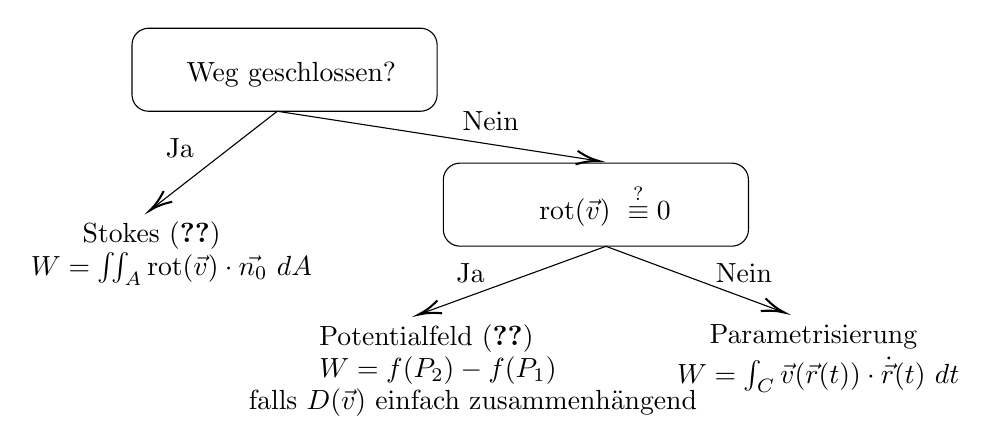
\begin{tikzpicture}[x=0.75pt,y=0.75pt,yscale=-1,xscale=1]
                \draw   (235,71) .. controls (235,66.58) and (238.58,63) .. (243,63) -- (374,63) .. controls (378.42,63) and (382,66.58) .. (382,71) -- (382,95) .. controls (382,99.42) and (378.42,103) .. (374,103) -- (243,103) .. controls (238.58,103) and (235,99.42) .. (235,95) -- cycle ;
                \draw   (385,136) .. controls (385,131.58) and (388.58,128) .. (393,128) -- (524,128) .. controls (528.42,128) and (532,131.58) .. (532,136) -- (532,160) .. controls (532,164.42) and (528.42,168) .. (524,168) -- (393,168) .. controls (388.58,168) and (385,164.42) .. (385,160) -- cycle ;
                \draw    (305,103) -- (245.25,149.5) ;
                \draw [shift={(243.67,150.73)}, rotate = 322.11] [color={rgb, 255:red, 0; green, 0; blue, 0 }  ][line width=0.75]    (10.93,-3.29) .. controls (6.95,-1.4) and (3.31,-0.3) .. (0,0) .. controls (3.31,0.3) and (6.95,1.4) .. (10.93,3.29)   ;
                \draw    (305,103) -- (458.02,126.69) ;
                \draw [shift={(460,127)}, rotate = 188.8] [color={rgb, 255:red, 0; green, 0; blue, 0 }  ][line width=0.75]    (10.93,-3.29) .. controls (6.95,-1.4) and (3.31,-0.3) .. (0,0) .. controls (3.31,0.3) and (6.95,1.4) .. (10.93,3.29)   ;
                \draw    (463.33,168.07) -- (374.88,200.31) ;
                \draw [shift={(373,201)}, rotate = 339.97] [color={rgb, 255:red, 0; green, 0; blue, 0 }  ][line width=0.75]    (10.93,-3.29) .. controls (6.95,-1.4) and (3.31,-0.3) .. (0,0) .. controls (3.31,0.3) and (6.95,1.4) .. (10.93,3.29)   ;
                \draw    (463.33,168.07) -- (547.46,199.3) ;
                \draw [shift={(549.33,200)}, rotate = 200.37] [color={rgb, 255:red, 0; green, 0; blue, 0 }  ][line width=0.75]    (10.93,-3.29) .. controls (6.95,-1.4) and (3.31,-0.3) .. (0,0) .. controls (3.31,0.3) and (6.95,1.4) .. (10.93,3.29)   ;

                % Text Node
                \draw (260,78) node [anchor=north west][inner sep=0.75pt]   [align=left] {Weg geschlossen?};
                % Text Node
                \draw (430,137) node [anchor=north west][inner sep=0.75pt]    {$\text{rot}(\vec{v}) \ \overset{?}{\equiv} 0$};
                % Text Node
                \draw (210,155) node [anchor=north west][inner sep=0.75pt]   [align=left] {Stokes (\ref{sec:SatzVonStokes})};
                % Text Node
                \draw (324,204.5) node [anchor=north west][inner sep=0.75pt]   [align=left] {Potentialfeld (\ref{sec:Potentialfeld})};
                % Text Node
                \draw (512,204.5) node [anchor=north west][inner sep=0.75pt]   [align=left] {Parametrisierung};
                % Text Node
                \draw (250,114.9) node [anchor=north west][inner sep=0.75pt]   [align=left] {Ja};
                % Text Node
                \draw (390,175) node [anchor=north west][inner sep=0.75pt]   [align=left] {Ja};
                % Text Node
                \draw (393,102) node [anchor=north west][inner sep=0.75pt]   [align=left] {Nein};
                % Text Node
                \draw (515,175) node [anchor=north west][inner sep=0.75pt]   [align=left] {Nein};
                % Text Node
                \draw (185,170) node [anchor=north west][inner sep=0.75pt]    {$W = \iint_{A} \text{rot}(\vec{v}) \cdot \vec{n_0} \ dA$};
                % Text Node
                \draw (324,220) node [anchor=north west][inner sep=0.75pt]    {$W = f(P_2) - f(P_1)$};
                \draw (290,235.5) node [anchor=north west][inner sep=0.75pt]    {falls $D(\vec{v})$ einfach zusammenhängend};
                % Text Node
                \draw (496.33,220) node [anchor=north west][inner sep=0.75pt]    {$W = \int_C \vec{v}(\vec{r}(t)) \cdot \dot{\vec{r}}(t) \ dt$};
            \end{tikzpicture}
        }
    
        % !TeX root = ../../ZF_bmicha_Ana.tex
\subsection{DGLs \& Vektorfelder}
    \vspace{0.5em}
    $$
    y' = \frac{v_2}{v_1} \qquad \vec{v} = \begin{pmatrix} v_1\\v_2 \end{pmatrix}
    $$
    \subsubsection{Feldlinien $y(x)$ $\to$ Vektorfeld $\vec{v}$}
        \begin{enumerate}
            \item Feldliniengleichung nach $x$ ableiten $\to$ $y'(x)$
            \item Scharparameter eliminieren
            \item $\displaystyle y' = \frac{v_2}{v_1}$ $\to$ $\vec{v} = \begin{pmatrix} v_1\\v_2 \end{pmatrix}$
        \end{enumerate}
    \subsubsection{Vektorfeld $\vec{v}$ $\to$Feldlinien $y(x)$}
        \vspace{0.5em}
        \begin{enumerate}
            \item $\displaystyle y' = \frac{v_2}{v_1}$
            \item DGL lösen
        \end{enumerate}
        \newpage

    \section{Differentialgleichungen (DGL)}
        % !TeX root = ../../ZF_bmicha_Ana.tex
\vspace{0.5em}
Potenzreihe der Funktion $f(x)$ um den Punkt $x_o$:
\mathbox{
    f(x) = \sum_{n=0}^{\infty} a_n \cdot (x-x_o)^n
}
\vspace{-1.0em}
\begin{itemize}
    \item Höchstens eine Potenzreihe von $f$ um $x_o$ existiert.
    \item Konvergiert für $\abs*{x-x_o} < r$
\end{itemize}
\vspace{-1em}
\mathbox{
    \frac{1}{1 - \fcolorbox{green}{white}{x}} = \sum\limits_{n = 0}^{\infty} \fcolorbox{green}{white}{x}^k
}
\vspace{-0.5em}
        \input{src/8_Differentialgleichungen/2_separierbare-DGL.tex}
        \input{src/8_Differentialgleichungen/3_substitutionen.tex}
        % !TeX root = ../../ZF_bmicha_Ana.tex
\subsection{Orthogonaltrajektorien}
    \mathbox{
        y' = - \frac{1}{y_{OT}'}
    }
    \begin{enumerate}
        \item Kurvenschar $y(x)$ ableiten $\to y'(x)$
        \item Scharparameter eliminieren
        \item Obige Relation einsetzen und $y \to y_{OT}$
        \item DGL für $y_{OT}$ lösen
    \end{enumerate}
        \input{src/8_Differentialgleichungen/5_enveloppe.tex}
        \input{src/8_Differentialgleichungen/6_linear-1-ordnung.tex}
        \input{src/8_Differentialgleichungen/7_spezielle-DGL.tex}
        \input{src/8_Differentialgleichungen/8_DGL-konst-Koeff.tex}
        \input{src/8_Differentialgleichungen/9_Lagrange-2-Ordnung.tex}
        \vfill \null \columnbreak
        \input{src/8_Differentialgleichungen/10_Euler-DGL.tex}
        \vfill \null \columnbreak
        \input{src/8_Differentialgleichungen/11_dgl_systeme.tex}
        \newpage

    \section{Appendix}
        \input{src/99_Appendix/nullstellen_reeller_polynome.tex}
        % !TeX root = ../../ZF_bmicha_Ana.tex
\subsection{Cosinus und Sinus - Integrale}
    Für $a,b \in \mathbb{Z}$ und $n \geq 2$, gelten:
    \begin{align*}
        \int_{a \cdot \frac{\pi}{2}}^{b \cdot \frac{\pi}{2}} \sin^n(x) \ dx 
            &= \frac{n-1}{n} \int_{a \cdot \frac{\pi}{2}}^{b \cdot \frac{\pi}{2}} \sin^{n-2}(x) \ dx\\[0.5em]
        \int_{a \cdot \frac{\pi}{2}}^{b \cdot \frac{\pi}{2}} \cos^n(x) \ dx 
            &= \frac{n-1}{n} \int_{a \cdot \frac{\pi}{2}}^{b \cdot \frac{\pi}{2}} \cos^{n-2}(x) \ dx
    \end{align*}
    Diese Regel kann mehrfach angewandt werden.
        \subsection{Polynome n-ten Grades}
    \begin{itemize}
        \item $f(x) = a \; \text{für alle} \; x \; \epsilon D(f) \; \Leftrightarrow f(x) \; \text{ist konstant}$
        \item $f'(x) \geq 0 \Leftrightarrow f(x) \; \text{ist monoton wachsend}$
        \item $f'(x) \leq 0 \Leftrightarrow f(x) \; \text{ist monoton fallend}$
        \item $f'(x) > 0 \Rightarrow f(x) \; \text{ist streng monoton wachsend}$
        \item $f'(x) < 0 \Rightarrow f(x) \; \text{ist streng monoton fallend}$
        \item $f''(x) > 0, x \; \epsilon \; [a,b] \Leftrightarrow f(x) \; \text{\textbf{konvex} auf} \; [a,b] \; \rotatebox[origin=c]{180}{$\curvearrowleft$}$
        \item $f''(x) < 0, x \; \epsilon \; [a,b] \Leftrightarrow f(x) \; \text{\textbf{konkav} auf} \; [a,b] \curvearrowright$
        \item $f^n(x):$
            \vspace*{-0.5em}
            \begin{itemize}
                \item $n$ ungerade $\rightarrow$ mind. eine Nullstelle
                \item maximal $n-1$ Extremalstellen
                \item $n$ gerade und $\geq 2 \rightarrow $ mind. eine Extremalstelle
                \item maximal $n-2$ Wendepunkte
                \item $n \geq 3$ und ungerade $\rightarrow$ mind. ein Wendepunkt, nicht zwingend Sattelpunkt
            \end{itemize}
    \end{itemize}
        \subsection{Wichtige Grenzwerte}
    \begin{minipage}{0.99\linewidth}
        \begin{minipage}{0.49\linewidth}
            \begin{align*}
                &\lim_{x \to 0} \frac{\arctan(x)}{x} &= 1\\
                &\lim_{x \to 0} \frac{\sin(x)}{x} &= 1\\
                &\lim_{x \to 0} \frac{\arcsin(x)}{x} &= 1\\
                &\lim_{x \to 0} \frac{x}{\sin(ax)} &= \frac{1}{a}\\
                &\lim_{x \to 0} \frac{\sin(ax)}{\sin(x)} &= a\\
                &\lim_{x \to 0} \frac{\ln(a+x)}{x} &= \frac{1}{a}\\
                &\lim_{x \to 0} \frac{\cos(x)-1}{x} &= 0\\
                &\lim_{x \to 0} \frac{1-\cos(x)}{x^2} &= \frac{1}{2}\\
                &\lim_{x \to 0} \frac{\tan(x)-1}{x} &= 1
            \end{align*}
        \end{minipage}
        \begin{minipage}{0.49\linewidth}
            \begin{align*}
                &\lim_{x \to \infty} x \cdot \sin{\frac{1}{x}} &= 1\\
                &\lim_{x \to \infty} a^{\frac{1}{x}} &= 1\\
                &\lim_{x \to \infty} x^{\frac{1}{x}} &= 1\\
                &\lim_{x \to \infty} \left(1+\frac{a}{x}\right)^x &= e^a\\
                &\lim_{x \to \infty} x^a \cdot \ln(x)^b &= 0\\
                &\lim_{x \to \infty} \frac{e^{ax}}{x^b} &= + \infty\\
                &\lim_{x \to \infty} \left(\frac{n-1}{n+1}\right)^n &= \frac{1}{e^2}\\
                &\lim_{x \to \infty} \frac{\ln(x)}{x-1} &= 1\\
                &\lim_{x \to \pm \pi/2} \frac{\tan(x)}{x} &= \mp \infty\\
            \end{align*}
        \end{minipage}
    \end{minipage}
        \subsection{Reihenentwicklung spezieller Funktionen}
    \vspace*{-0.5em}
    \begin{align*}
        \frac{1}{1-x} &= \sum_{n=0}^\infty x^n = 1 + x + x^2 + \dots\\
        \frac{1}{1+2x^2} &= \sum_{n=0}^\infty (-2x^2)^n = 1 - 2x^2 + 4x^4 + \dots\\
        \frac{x^2}{5-x} &= x^2 \cdot \frac{1}{5} \cdot \sum_{n=0}^\infty \left( \frac{x}{5} \right)^n = \sum_{n=0}^\infty \left( \frac{1}{5} \right)^{n+1} x^{n+2}\\
        e^x &= \sum_{n=0}^\infty \frac{x^n}{n!} = 1 + x + \frac{x^2}{2!} + \frac{x^3}{3!} + \dots\\
        \sin(x) &= \sum_{n=0}^\infty (-1)^n \cdot \frac{x^{2n+1}}{(2n+1)!} = x - \frac{x^3}{3!} + \frac{x^5}{5!} - \dots
    \end{align*}
        \subsection{Wichtige Integrale}
    \begin{align*}
        &\int \sin(x) \cos(x) dx = - \frac{1}{2} \cos^2(x) + C\\
        &\int \sin^2(x) \cos(x) dx = \frac{1}{3} \sin^3(x) + C\\
        &\int \sin(x) \cos^2(x) dx = - \frac{1}{3} \cos^3(x) + C\\
        &\int \ln(x) dx = x(\ln(x) -1) + C\\
        &\int \frac{1}{x \ln(x)} dx = \ln|\ln|x|| + C\\
        &\int 2x \sqrt{r^2 - x^2} dx = -\frac{2}{3} (r^2-x^2)^\frac{3}{2} + C, \; r \neq 0\\
        &\int \sqrt{1+x^2} dx = \frac{1}{2} \left(\textrm{Arsinh}(x) + x \sqrt{1+x^2}\right) + C\\
        &\int \sqrt{1-x^2} dx = \frac{1}{2} \left(\arcsin(x) + x \sqrt{1-x^2}\right) + C\\
        &\int \frac{x}{\sqrt{x^2-1}} dx = \sqrt{x^2-1} + C\\
        &\int \frac{x}{\sqrt{x^2+1}} dx = \sqrt{x^2+1} + C\\
        &\int \frac{1}{x^2+x} dx = -\ln|1+x^-1| + C\\
    \end{align*}
        % !TeX root = ../../ZF_bmicha_Ana.tex
\subsection{Ableitung Un-/Gerader Funktionen}
\begin{itemize}
    \item $g(x)$ sei \textbf{gerade}
        $$
            g'(0)=g^{(3)}(0)=g^{(5)}(0)=...=0
        $$
    \item $f(x)$ sei \textbf{ungerade}
        $$
            f''(0)=f^{(4)}(0)=f^{(6)}(0)=...=0
        $$
\end{itemize}
        \input{src/99_Appendix/exponentialgesetze.tex}
        \subsection{Polarkoordinaten}
    Umrechnung im ersten Quadranten
    \begin{align*}
        \begin{rcases}
            r = \rho(\phi)\\
            x = \cos(\phi) \cdot r\\
            y = \sin(\phi) \cdot r
        \end{rcases} \phi \in \left[0, \frac{\pi}{2}\right]
    \end{align*}
        \subsection{Häufige Parametrisierungen}
    \subsubsection{Ellipse}
    \vspace{0.5em}
    \mathbox{
        \overrightarrow{r}(t) = \binom{a \cdot cos(t) + x_0}{b \cdot sin(t) + y_0}
    }
    \text{Sonderfall Kreis mit Radius } a = b
    \begin{center}
        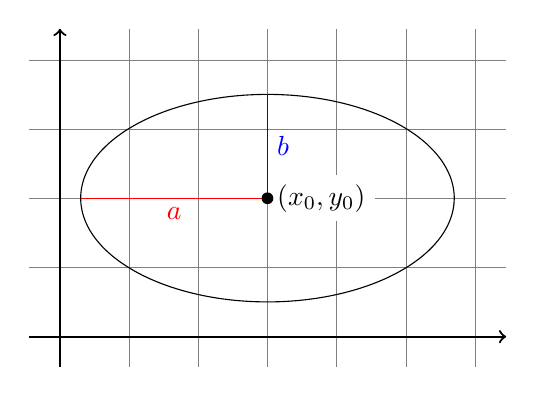
\begin{tikzpicture}[x=0.75pt,y=0.75pt,yscale=-1,xscale=1]
            %coordinatum system
            \foreach \i in {0, ..., 6} {
                \draw [very thin,gray] (\i * 33.33, -15) -- (\i * 33.33, 148);
            }
            \foreach \i in {0, ..., 4} {
                \draw [very thin,gray] (-15 ,\i * 33.33) -- (215 ,\i * 33.33);
            }
            \draw[thick, <-] (0, -15) -- (0, 148);
            \draw[thick, ->] (-15, 133.33) -- (215, 133.33);
            %
            %Ellipse
            \draw plot [smooth, samples = 100, domain = 0:500] ({90 * cos(\x) + 100}, {50 * sin(\x) + 66.6});
            %a
            \draw [red] (100, 66.66) -- (55, 66.66) node[anchor = north, red] {$a$} -- (10, 66.66);
            %b
            \draw [blue] (100, 66.66) -- (100, 41.66) node[anchor = west, blue] {$b$} -- (100, 16.66);
            %Midpoint
            \draw (100, 66.66) node[right, fill=white] {$(x_0, y_0)$} node[circle, fill, inner sep = 1.5pt]{};
        \end{tikzpicture}\\
    \end{center}
    
    \subsubsection{Zykloide}
    \vspace{0.5em}
    \mathbox{
        \overrightarrow{r}(t) = \binom{rt - a \sin(t)}{r - a \cos(t)}
    }
    \text{Sonderfall Gewöhnliche Zykloide } r = a\\
    \begin{center}
        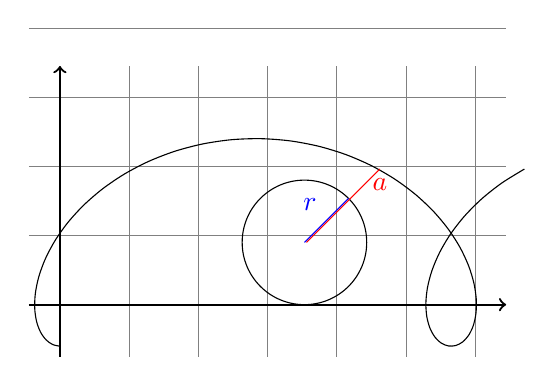
\begin{tikzpicture}[x=0.75pt,y=0.75pt,yscale=1,xscale=1]
            %coordinatum system
            \foreach \i in {0, ..., 6} {
                \draw [very thin,gray] (\i * 33.33, -25) -- (\i * 33.33, 115);
            }
            \foreach \i in {0, ..., 4} {
                \draw [very thin,gray] (-15 ,\i * 33.33) -- (215 ,\i * 33.33);
            }
            \draw[thick, ->] (0, -25) -- (0, 115);
            \draw[thick, ->] (-15, 0) -- (215, 0);
            %
            %Zykloide
            \draw plot [smooth, variable=\x, domain=0:2.75*pi, samples = 50] ({30 * \x - 50 * sin(\x*180/pi)},{30 - 50 * cos(\x*180/pi)});
            %circle
            \draw ({30 * (1.25 * pi)}, 30) circle (30);
            %a
            \draw [red] ({1 + 30 * (1.25 * pi)}, 30) -- ({1 + 30 * (1.25 * pi) - 50 * sin((1.25 * pi)*180/pi)}, {30 - 50 * cos((1.25 * pi)*180/pi)}) node[anchor = north, red] {$a$};
            %radius
            \draw [blue] ({30 * (1.25 * pi)}, 30) -- ({(30 * (1.25 * pi) + 30 * (1.25 * pi) + 30 * 1.414/2)/2}, {(30 + 30 + 30 * 1.414/2)/2}) node[anchor = south east, blue] {$r$} -- ({30 * (1.25 * pi) + 30 * 1.414/2}, {30 + 30 * 1.414/2});
            %
        \end{tikzpicture}\\
    \end{center}

    \vfill \null \columnbreak

    \subsubsection{Epizykloide}
    \vspace{0.5em}
    \mathbox{
        \overrightarrow{r}(t) = \binom{R cos(t) - a cos(\frac{R}{r} t)}{R sin(t) - a sin(\frac{R}{r} t)}
    }
    \text{Sonderfall Kardioide } R = 2r, r = a\\
    \begin{center}
        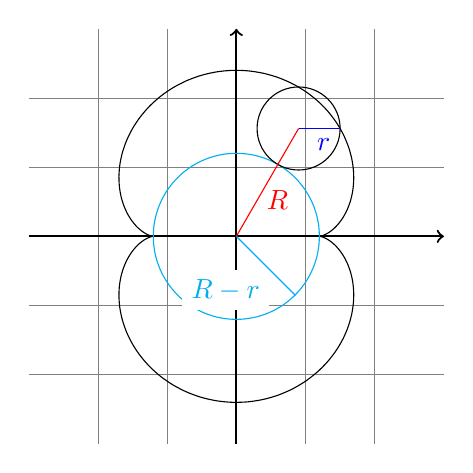
\begin{tikzpicture}[x=0.75pt,y=0.75pt,yscale=1,xscale=1]
            %coordinatum system
            \foreach \i in {-2, ..., 2} {
                \draw [very thin,gray] (\i * 33.33, -100) -- (\i * 33.33, 100);
            }
            \foreach \i in {-2, ..., 2} {
                \draw [very thin,gray] (-100 ,\i * 33.33) -- (100 ,\i * 33.33);
            }
            \draw[thick, ->] (0, -100) -- (0, 100);
            \draw[thick, ->] (-100, 0) -- (100, 0);
            %
            %Epizykloide
            \draw plot [smooth, variable=\x, domain=0:2*pi, samples = 100] ({60 * cos(\x*180/pi) - 20 * cos(60/20 * \x*180/pi)},{60 * sin(\x*180/pi) - 20 * sin(60/20 * \x*180/pi)});
            %big circle
            \draw [cyan] (0, 0) circle (40);
            \draw [cyan] (0, 0) -- (1.424/4 * 45, -1.424/4 * 45) node[anchor = north east, cyan, fill=white] {$R-r$} -- (1.424/2 * 40, -1.424/2 * 40);
            %small circle (t = pi/3)
            \draw ({60 * cos(60)}, {60 * sin(60)}) circle (20);
            %R
            \draw [red] (0, 0) -- ({20 * cos(60)}, {20 * sin(60)}) node[anchor = west, red] {$R$} -- ({60 * cos(60)}, {60 * sin(60)});
            %r
            \draw [blue] ({60 * cos(60)}, {60 * sin(60)}) -- ({60 * cos(60) - 20 * cos(60/20 * 60)},{60 * sin(60) - 20 * sin(60/20 * 60)}) node[anchor = north east, blue] {$r$};
            %
        \end{tikzpicture}\\
    \end{center}

    \subsubsection{Hypozykloide}
    \vspace{0.5em}
    \mathbox{
        \overrightarrow{r}(t) = \binom{R cos(t) + a cos(\frac{R}{r} t)}{R sin(t) - a sin(\frac{R}{r} t)}
    }
    \begin{center}
        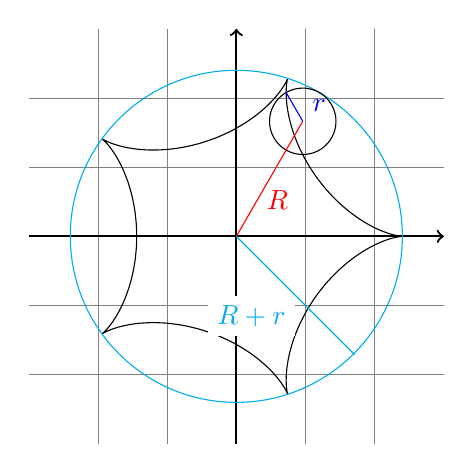
\begin{tikzpicture}[x=0.75pt,y=0.75pt,yscale=1,xscale=1]
            %coordinatum system
            \foreach \i in {-2, ..., 2} {
                \draw [very thin,gray] (\i * 33.33, -100) -- (\i * 33.33, 100);
            }
            \foreach \i in {-2, ..., 2} {
                \draw [very thin,gray] (-100 ,\i * 33.33) -- (100 ,\i * 33.33);
            }
            \draw[thick, ->] (0, -100) -- (0, 100);
            \draw[thick, ->] (-100, 0) -- (100, 0);
            %
            %Hypozykloide
            \draw plot [smooth, variable=\x, domain=0:2*pi, samples = 100] ({64 * cos(\x*180/pi) + 16 * cos(64/16 * \x*180/pi)},{64 * sin(\x*180/pi) - 16 * sin(64/16 * \x*180/pi)});
            %big circle
            \draw [cyan] (0, 0) circle (80);
            \draw [cyan] (0, 0) -- (1.424/4 * 80, -1.424/4 * 80) node[anchor = north east, cyan, fill=white] {$R+r$} -- (1.424/2 * 80, -1.424/2 * 80);
            %small circle (T = pi/3)
            \draw ({64 * cos(60)}, {64 * sin(60)}) circle (16);
            %R
            \draw [red] (0, 0) -- ({20 * cos(60)}, {20 * sin(60)}) node[anchor = west, red] {$R$} -- ({64 * cos(60)}, {64 * sin(60)});
            %r
            \draw [blue] ({64 * cos(60)}, {64 * sin(60)}) node[anchor = south west, blue] {$r$} -- ({64 * cos(60) + 16 * cos(64/16 * 60)},{64 * sin(60) - 16 * sin(64/16 * 60)});
            %
        \end{tikzpicture}\\
    \end{center}

    \subsubsection{Lissajous-Figuren}
    \vspace{0.5em}
    \mathbox{
        \overrightarrow{r}(t) = \binom{a_1 sin(\omega_1 t + \varphi_1)}{a_2 sin(\omega_2 t + \varphi_2)}
    }
        \subsection{Häufige Funktionsgraphen}
    \centerline{
        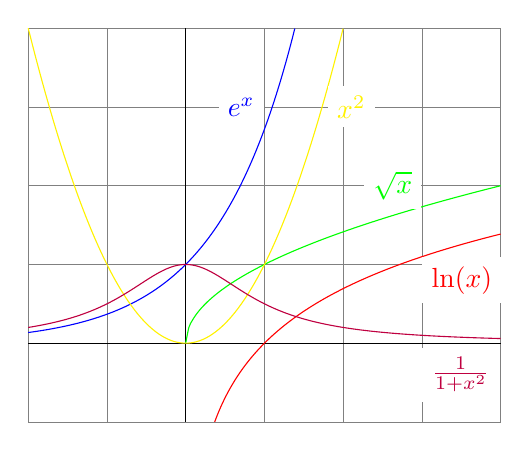
\begin{tikzpicture}
            \draw [help lines] (-2,-1) grid [step=1] (4,4);
            \draw (-2,0) -- (4,0);
            \draw (0,-1) -- (0,4);
            \draw [color = red] plot [smooth, samples = 100, domain = 0.368:4] (\x, {ln(\x)});
                \draw (3, 0.8) node[right, red, fill=white] {$\ln(x)$};
            \draw [color = blue] plot [smooth, samples = 100, domain = -2:1.386] (\x, {e^\x});
                \draw (1,3) node[left, blue, fill=white] {$e^x$};
            \draw [color = green] plot [smooth, samples = 100, domain = 0:4] (\x, {sqrt(\x)});
                \draw (3,2) node[left, green, fill=white] {$\sqrt{x}$};
            \draw [color = yellow] plot [smooth, samples = 100, domain = -2:2] (\x, {(\x)^2});
                \draw (1.8, 3) node[right, yellow, fill=white] {$x^2$};
            \draw [color = purple] plot [smooth, samples = 100, domain = -2:4] (\x, {1/(1+(\x)^2)});
                \draw (3,-0.4
                ) node[right, purple, fill=white] {$\frac{1}{1+x^2}$};
        \end{tikzpicture}
    }
        \vfill \null \columnbreak
        % !TeX root = ../../ZF_bmicha_Ana.tex
\subsection{Schwerpunkt / Trägheitsmoment}
    Sei $H(x)$ die Höhe des Fläche a.d.S. $x$.\\
    Sei $\sigma$ die Flächendichte $[kg/m^2]$.
    \begin{align*}
        \textrm{Fläche: }  A = \int_{x_1}^{x_2} H(x)\ dx\\
        \textrm{Masse: }  M = \int_{x_1}^{x_2} \sigma \cdot H(x)\ dx\\
        \textrm{Schwerpunkt: }  x_s = \frac{1}{M} \int_{x_1}^{x_2} x \cdot \sigma \cdot H(x)\ dx\\
        \textrm{SP Rotationsvolumen: } x_s = \frac{1}{V} \int_{x_1}^{x_2} x \cdot \pi \cdot H^2(x)\ dx\\
        \textrm{Trägheitsmoment: }  I_y = \int_{x_1}^{x_2} x^2 \cdot \sigma \cdot H(x)\ dx
    \end{align*}
    \subsubsection{Trägheitsmoment}
    \vspace*{-1em}
        \begin{align*}
            \Theta =& \int (\textrm{Abstand zur Rotationsachse})^2 \cdot (\textrm{Masse})\\
            \Theta =& \; \rho \cdot \int_a^b x^2 \cdot G(x) dx\\
            J_0 =& \; \frac{\pi R^4}{2} = \; \parbox{5cm}{polares Flächenträgheitsmoment\\ der Kreisscheibe}\\
            \Theta_x =& \; \rho \cdot \int_a^b \frac{1}{2} \pi (f(x))^4 dx = \; \parbox{5cm}{Masseträgheitsmoment\\ eines Rotationskörpers\\ um die x-Achse}\\
            \Theta =& \; \rho \cdot \frac{1}{2} \pi \int_a^{b} y(t)^4\|\dot{x}(t)\| dt\\
            G(x) =& \; \text{Masse an diesem Abstand}\\
            M(x) =& \; \text{Mantelfäche} = 2 \pi x \cdot G(x) = \text{Umfang} \cdot \text{Höhe}\\ %\underbrace{2 \pi x \vphantom{G(x)}}_{\text{Umfang}} \cdot \underbrace{G(x)}_{\text{Höhe}}\\
            \Theta_z =& \; \rho \int_{x_1}^{x_2} x^2 \cdot M(x) dx
        \end{align*}        
\end{document}